

\part{Training Critique Models to Assist Coding Agents}
\label{part:usage}


\start{Overview of Part~\ref{part:usage}}
In \autoref{part:scalability} and \autoref{part:generalizability}, we aim to construct synthetic data to improve coding agent effectiveness. However, such methods are inherently bottlenecked by the capacity of the base models.
To address this limitation, in this part, we develop an auxiliary model to assist the primary coding agent. With the auxiliary model in the context, the search space of the coding agent's actions is reduced. Therefore the system can achieve potentially better performance with the same capacity of the coding agent.

Specifically, we identify two key principles that an ideal auxiliary model should follow: (1) it should provide additional performance gains when collaborating with the primary coding agent, and (2) it should specialize in capabilities that are different from the main coding agent.
We then show that a critique model that is trained to provide textual critiques for the main model during inference can achieve both principles, for both seq-to-seq NLP tasks (\autoref{chap:fence}) and coding agent tasks (\autoref{chap:prm-training}).

In \autoref{chap:fence}, we show that a critique model can improve the factuality of a generator model by either interacting with it in inference or providing feedback to assist training. We further improve the effectiveness of the critique model by constructing tailored training data.

When it comes to the domain of coding agent, in a \proposedWork (\autoref{chap:prm-training}), we first show that using a frontier model (e.g., Claude) to provide critique during inference substantially improves the correctness of a coding agent. Then we distill a more cost-efficient critique model by constructing synthetic supervised-finetuning training data. To further improve its effectiveness, we propose a method to construct direct preference optimization (DPO) training data, focusing on its gap between the frontier critique model.



\chapter{Improving Generator Factuality by Training an Evaluator Model}
\label{chap:fence}

\begin{figure}[t]
\centering
    \centering
    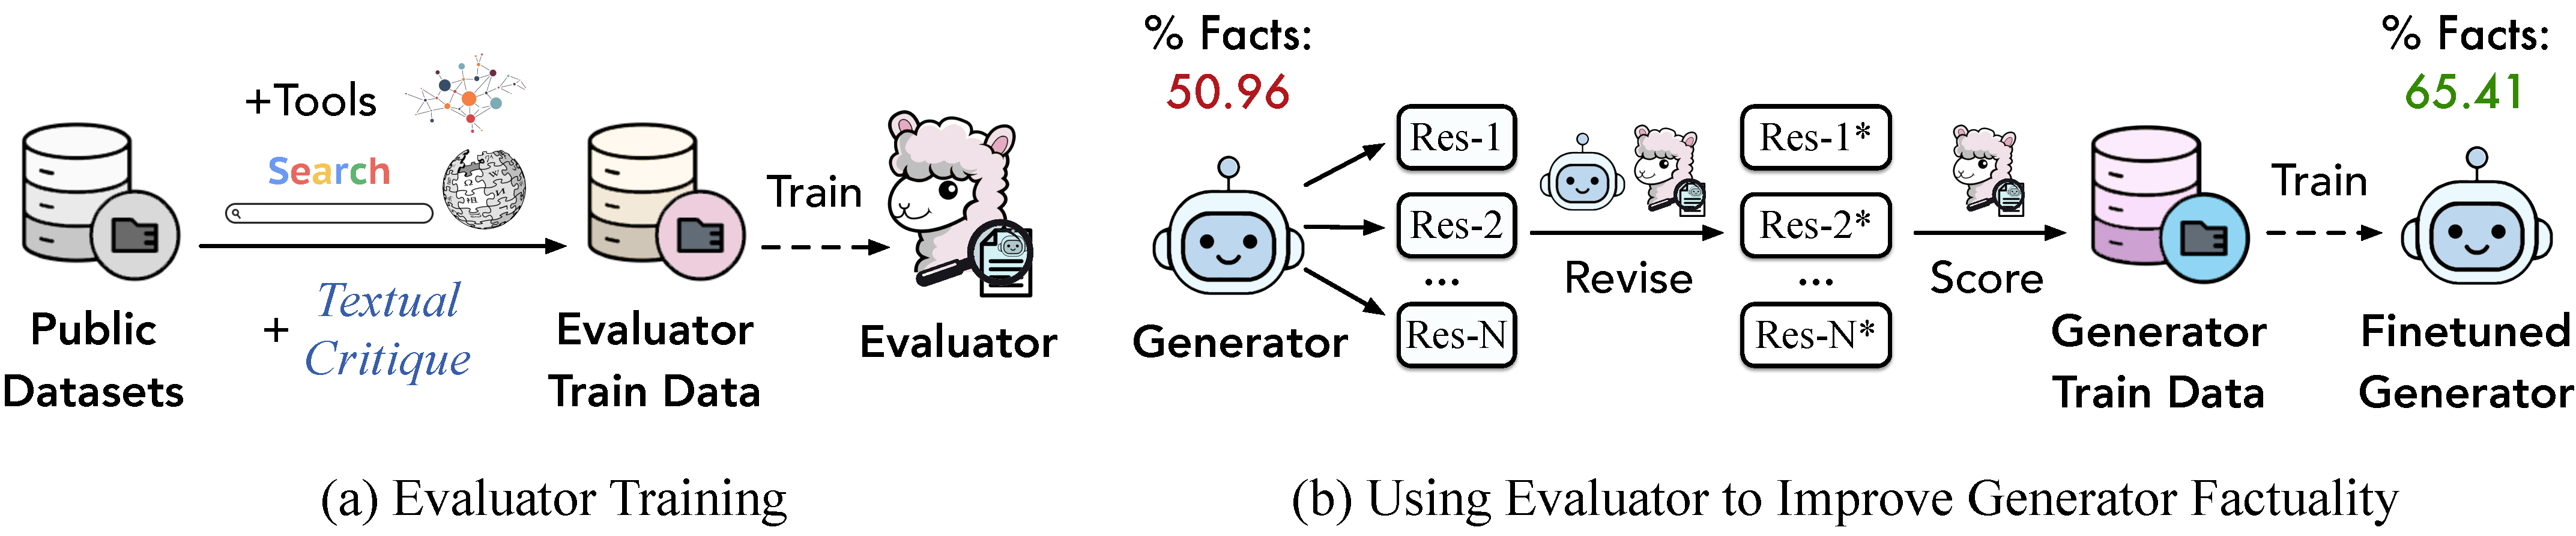
\includegraphics[width=\linewidth]{FenCE_figures/overall.pdf}
    \upv
    \caption{\textit{(Left)} The framework to train an evaluator, \fencemodelname, by augmenting public datasets with textual critiques and more diverse knowledge sources. We show the details in \autoref{fig:evaluator_train}.
    \textit{(Right)} The framework to improve model factuality with \fencemodelname. We construct training data by leveraging \fencemodelname to revise and score the generator's responses. Details of response revision are shown in \autoref{fig:revise}.}
    \label{fig:overview}
    \downv
\end{figure}

\section{Introduction}
Hallucination is one of the persistent challenges for large language models (LLMs), where models generate plausible-sounding but incorrect information, even if they are shown factual information during pretraining~\citep{hallucination-survey,empirical-factuality}. 
One hypothesis is that LLMs fail to distinguish the boundary between memorized facts and other plausible-sounding information and do not learn to only output memorized facts, especially on their unfamiliar topics~\citep{finetuning-on-new,understand-finetuning,unfamiliar-finetuning}.
Although it is possible to reduce hallucination in inference with decoding strategies~\citep{ITI,DoLA} or post-editing~\citep{FAVA,EVER}, they introduce severe latency issues and hurts efficiency in real-time applications.


Alternatively, prior studies train the generator to output more factual responses, by preferring (1)  generation candidates with higher factuality scores \citep{FactTune}, which is limited by the generator's capabilities, or (2) responses with false information corrected~\citep{EVER}, 
which is prone to introducing lesser-known facts.
As shown in recent work~\citep{finetuning-on-new,understand-finetuning}, such preference training reinforces the model to generate information not well memorized during pretraining, and hence could even hurt factuality.
Furthermore, the methods either leverage proprietary models that have restricted terms of use, or prompt the generator to evaluate its own factuality, which suffers from self-bias and leads to inaccurate judgments~\citep{self-bias}.


Recent work trains evaluator models that could potentially be used to provide training signals for generators.
One category of work relies on proprietary models (e.g., GPT-4) to generate training data in various formats~\citep{prometheus,AutoJ}.
In contrast, \citet{FLAMe} leverage public datasets containing judgments of whether a claim is factual against certain source documents. 
However, such documents are generally sampled from very \textbf{restricted sources} such as news corpora or Wikipedia, while an evaluator could potentially benefit from knowledge obtained by a multiplicity of tools (e.g., search engines)~\citep{longform}.
Furthermore, the judgment label in most datasets is a single binary or numeric score, providing \textbf{limited feedback} to the generator model.

In this paper, we present \fencemodelname, a \textbf{F}in\textbf{e}-grai\textbf{n}ed \textbf{C}ritic-based \textbf{E}valuator that aims to provide textual critiques for each model-generated claim based on diverse knowledge sources.
We start with a set of public datasets with human judgments on the factuality of model-generated claims. 
As shown in \autoref{fig:overview}(a), we augment the judgment labels with textual critiques, which provide more informative and explainable feedback to the generator.
In addition, we augment the source documents by invoking multiple tools, including a search engine, knowledge base, and knowledge graph, with the goal of training the evaluator to leverage more diverse knowledge sources.

We further demonstrate how to leverage \fencemodelname to improve the generator's factuality with finetuning.
To construct training data (\autoref{fig:overview}(b)), we generate multiple responses for each prompt, use \fencemodelname to judge and critique every claim in the responses, and replace false information with facts or remove it from the response, depending on whether the corresponding fact is within the generator's knowledge 
(i.e., whether the generator outputs \textit{``unknown''} when prompted about claim correctness). 
This mitigates introducing lesser-known facts into training data.
% \dpfried{this is interesting! People might wonder how it's done. Is it possible to convey this using just a few words?}
Finally, unlike existing work that use the generator itself as the evaluator, we use \fencemodelname to score each original and revised response and construct preference data, which reduces self-bias and produces more accurate judgments.


Experiments show that \fencemodelname outperforms large open-source models such as Mistral-123B and strong proprietary models such as Claude-3 on LLM-Aggrefact.
With \fencemodelname, we improve Llama2-7B-chat's factuality by 16.86\% on FActScore~\citep{factscore} and 17.64\% on TruthfulQA \cite{truthfulqa}, outperforming existing factuality finetuning methods by 8.83\% and 3.99\%, respectively.
Analyses further show that after training with our recipe, the generator outputs less information for unfamiliar entities and more information for popular ones, suggesting that it learns to only generate information that is likely to be factual.

\start{Contributions}
(1) We train a fine-grained critique-based evaluator, \fencemodelname, by augmenting public datasets with textual critiques and more diverse source documents.
(2) We propose a training recipe to improve the generator's factuality by leveraging \fencemodelname to improve and score its responses.
(3) We conduct extensive experiments to validate both the judgment accuracy of \fencemodelname and the factuality of the generator trained with \fencemodelname, outperforming state-of-the-art factuality training methods by 8.83\% on FActScore and 3.99\% on TruthfulQA.





\section{Methodology}

\begin{figure}[t]
\centering
    \centering
    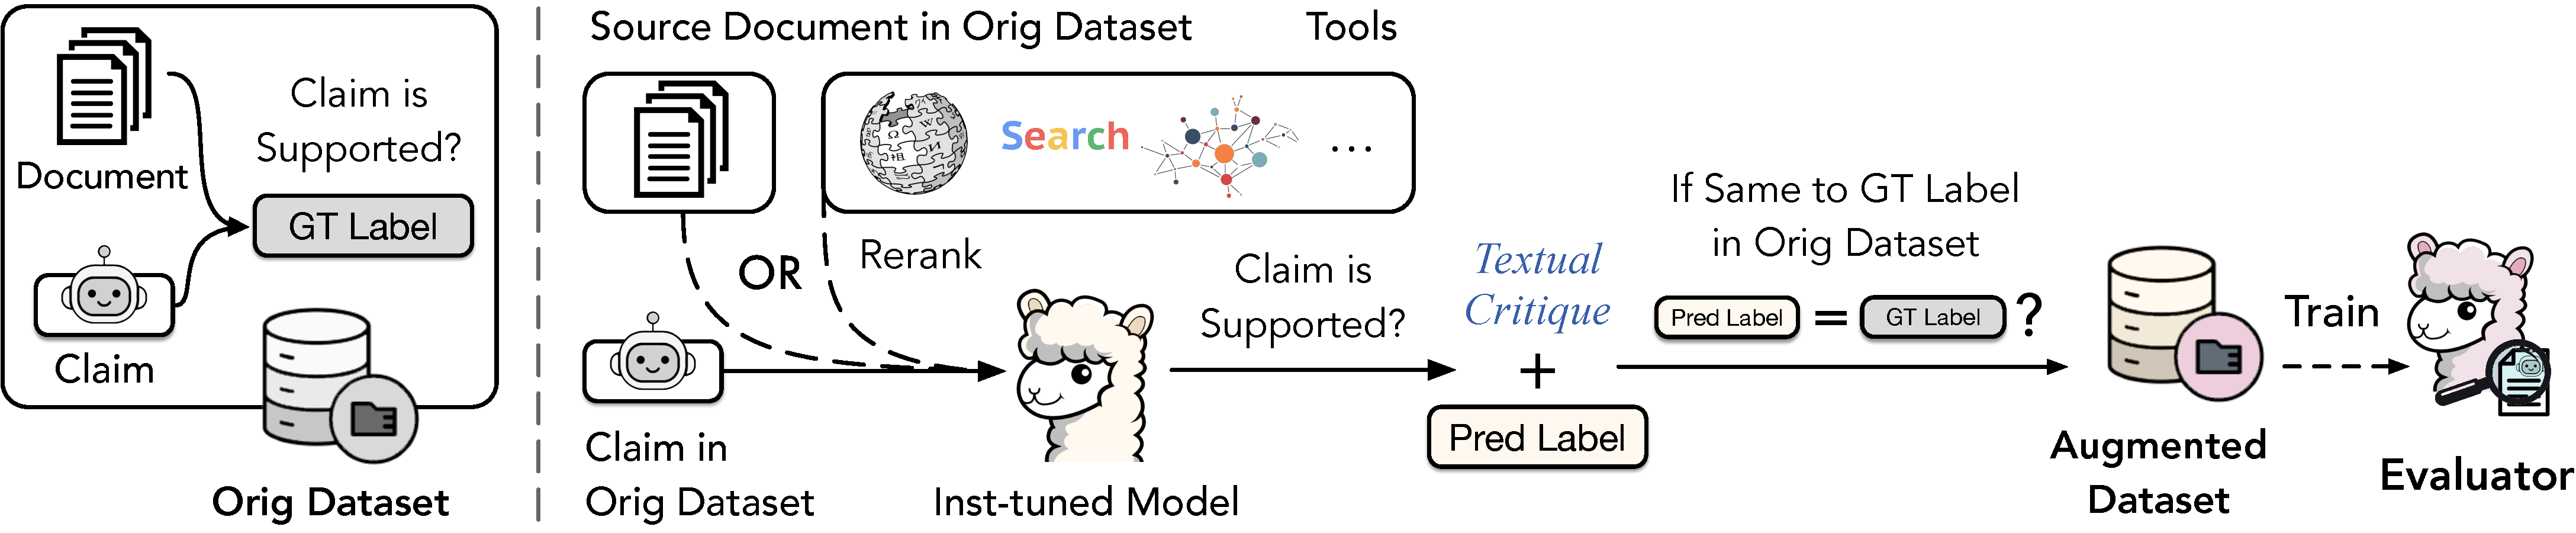
\includegraphics[width=\linewidth]{FenCE_figures/evaluator_train.pdf}
    \upv
    \caption{Framework of evaluator training. (\textit{left}) Existing public datasets for evaluator training. Each example contains a claim, a source document, and the ground truth (GT) label of whether the claim is supported by the document. (\textit{Right}) We augment the datasets with textual critiques and more diverse source documents obtained by tools. We use zero-shot Llama-3-70B-chat as the instruction-tuned model in our experiments.}
    \label{fig:evaluator_train}
    \downv
\end{figure}

\subsection{\fencemodelname: Factuality Evaluator Training}
\label{sec:evaluator_training}

\start{Preliminary}
To train the evaluator to recognize hallucinations, previous work~\citep{FLAMe} incorporates a combination of datasets with human judgments on factuality. As shown in \autoref{fig:evaluator_train}, in most datasets, each example contains a claim, a source document, and the ground-truth judgement of whether the claim is (1) fully supported by, (2) contradicted with, or (3) contains information that cannot be verified by the document.



We formally define the problem as follows:
Given a claim $c \in \mathcal{C}$, a source document $d \in \mathcal{D}$, a factuality evaluator aims to learn a mapping $f: \mathcal{C} \times \mathcal{D} \rightarrow \mathcal{L}$, which maps each claim-document pair $(c,d)$ to one of the labels:  
$f(c,d) = l \in \mathcal{L} =$ \{\textit{Supported, Contradictory, Unverified}\}.



\start{Augmenting Labels with Textual Critiques}
In addition to the classification label, we aim to train the evaluator to generate a \textit{textual critique} that explains the judgement, which provides more informative feedback such as which part of the document supports or contradicts the claim. We will leverage such feedback to revise generator responses and use them to train a more factual generator (see \S\ref{sec:improve_factuality} for details).
Formally, we aim to learn the mapping $f: \mathcal{C} \times \mathcal{D} \rightarrow \mathcal{R} \times \mathcal{L}$, which maps each claim-document pair $(c,d)$ to both the textual critique $r \in \mathcal{R}$ and the label $l \in \mathcal{L}$.


As shown in \autoref{fig:evaluator_train}, we prompt an instruction-tuned model $\mathcal{M}$ (e.g., Llama3-70B-chat) to generate both the critique $r_\mathcal{M}$ and label $l_\mathcal{M}$ for whether a claim $c$ is supported. The critique and label are likely to be consistent because the label is generated conditioned on the critique. As a result, if the predicted label $l_\mathcal{M}$ aligns with the ground truth label $l_{GT}$ in the original dataset, the critique is also likely to be aligned and we hence use both the critique $r_\mathcal{M}$ and label $l_\mathcal{M}$ as the new training target. Otherwise, if the predicted label does not align with the ground truth, we discard the whole example.



\start{Augmenting Source Documents using Tools}
To judge the factuality of an arbitrary model-generated claim, we could potentially benefit from \textit{a multiplicity of tools} such as search engines or online knowledge bases. However, the source documents in existing judgment datasets typically come from very restricted sources, such as news corpora or Wikipedia.
To bridge this gap, we obtain additional source documents for each claim by calling the following tools: a search engine (Bing Search API), knowledge base (Wikipedia), and knowledge graph (Google Knowledge Graph API).


As shown in \autoref{fig:evaluator_train}, given the claim $c$ in the original dataset, we prompt an instruction-tuned model to call multiple tools to verify the factuality of the claim (i.e., by generating tool calls such as search queries).
Then we rerank the returned results to obtain a combination of tool-extracted documents $d_t$. 
Similar to critique generation, we prompt the instruction-tuned model $\mathcal{M}$ to predict whether claim $c$ is supported by the tool-extracted documents $d_t$. We add $d_t$ to the train set if the predicted label $f_\mathcal{M}(c, d_t)$ is the same as the ground truth label $f_{GT}(c, d)$ in the original dataset.

The intuition is that if a claim can be supported by some documents, it is likely that we can obtain other supporting sources by calling the tools.
If a claim is hallucinated, it is very unlikely to find any knowledge that supports it with any tools. In both cases, we have $f_{GT}(c, d_t) = f_{GT}(c, d)$.



\start{Training Objective}
After obtaining the augmented training data $\mathcal{TR}_{Eval}=\{(c,d),(r,l)\}$, where each example contains (claim $c$, source document $d$, critique $r$, label $l$), we initialize the evaluator $\mathcal{E}$ with a instruction-tuned model and train it with a standard conditional language modeling objective, maximizing likelihood:
\begin{equation}
    \max _{\mathcal{E}} \mathbb{E}_{(c,d),(r,l) \sim \mathcal{TR}_{Eval}} \log \mathbb{P}_{\mathcal{E}}(r, l \mid c, d).
\label{eq:evaluator_sft}
\end{equation}


\begin{figure}[t]
\centering
    \centering
    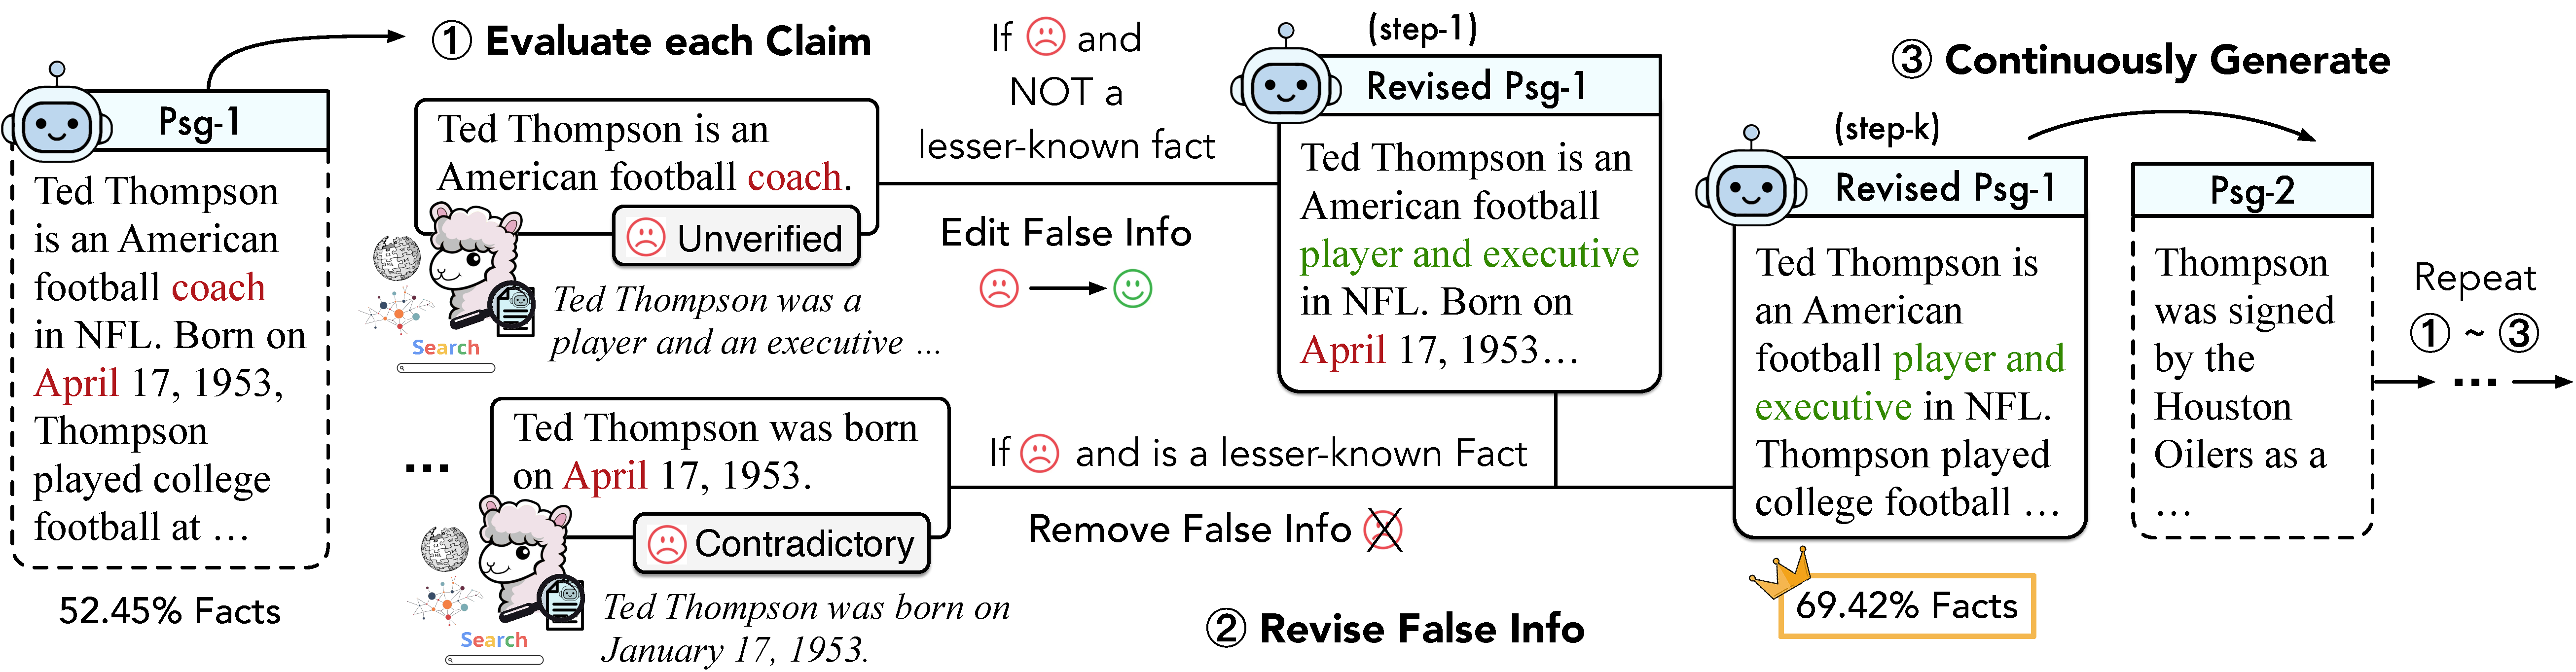
\includegraphics[width=\linewidth]{FenCE_figures/improve_factuality_v2.pdf}
    \upv
    \caption{
    The framework to revise model responses without introducing lesser-known facts. 
    We iteratively 
    (1) use \fencemodelname to evaluate the factuality of each claim, 
    (2) replace false information (if any) with the correct fact or remove it from the response, depending on whether it corresponds to a lesser-known fact,
    and (3) continue generating the next passage. 
    For every claim, we prompt the generator ``\textit{Is this claim factual?}'' without providing any source documents. If the generator outputs \textit{``unknown''}, we assume that the claim corresponds to a lesser-known fact.
    }
    \label{fig:revise}
    \downv
\end{figure}


\subsection{Improving Generator Factuality with \fencemodelname}
\label{sec:improve_factuality}
In this section, we use our evaluator, \fencemodelname, to improve a generator model's factuality, where we construct training data by revising and scoring the generator's own responses.
Compared to directly training the generator on factuality datasets, our method only requires a prompt set as inputs and hence enjoys much better scalability.

\start{Overview}
As shown in \autoref{fig:overview}, given a prompt, we use the generator to generate $N$ candidate responses.
Then we improve the factuality of each response by using \fencemodelname to evaluate the factuality of each piece of generated information and editing or removing the false information, depending on whether the corresponding fact is rare.
Finally, we use \fencemodelname again to score all original and revised responses and construct training data.

\start{Response Revision}
We aim to improve the factuality of the generator's responses \textit{without introducing lesser-known facts} to training data. The motivation is that as shown in recent research~\citep{understand-finetuning,finetuning-on-new}, forcing the model to generate lesser-known facts that are poorly memorized during pretraining will blur the boundary with memorized facts and other plausible sounding information, which may lead to even more hallucination.
As shown in \autoref{fig:revise}, we iteratively revise each passage with the following three steps: 

\quad [\underline{\textbf{Step}-\circled{1} \textbf{Evaluate}}] 
we prompt an instruction-tuned model (e.g., Llama3-70B-chat) to decompose each response into claims. Then for each claim, we call tools to obtain related documents and apply \fencemodelname to evaluate its factuality with critique. 

\quad [\underline{\textbf{Step}-\circled{2} \textbf{Revise}}] 
If there are any claims that are judged as \textit{``unverified''} or \textit{``contradictory,''} we further check whether it corresponds to a lesser-known fact. 
Specifically, we prompt the generator \textit{``Is this claim factual?''} and output \textit{``true,''} \textit{``false,''} or \textit{``unknown,''} without providing it any external knowledge. We regard the claim as a lesser-known fact if the generator outputs \textit{``unknown.''}

If the claim does not correspond to a lesser-known fact, we prompt the generator to correct the false information based on the critique generated by \fencemodelname. Otherwise, we prompt the generator to remove the false information from the passage.

\quad [\underline{\textbf{Step}-\circled{3} \textbf{Generate}}] 
To reduce error propagation, we use the revised passages as the prefix and continuously generate the next passage.


\start{Generator Training}
We use \fencemodelname to score each original and revised response by computing the percentage of factual claims. Then we train the generator with first supervised finetuning (SFT) and then direct preference optimization (DPO)~\citep{DPO}.
In the SFT stage, we train the generator with the top-$k$ responses as targets, where the responses are ranked by the percentage of factual claims, optimizing with the conditional language modeling objective, which is similar to \autoref{eq:evaluator_sft}.

In the DPO stage~\citep{DPO}, we construct preference data $\mathcal{TR}_{Gen}= \{x, y_w, y_l\}$ as follows: for each prompt $x$, we choose the preferred response $y_w$ from the top-$k$ responses and choose any responses with lower scores than $y_w$ as the rejected response $y_l$.
Suppose we have $N$ original and $N$ revised responses, this gives us $\binom{2N}{2} - \binom{2N-k}{2}$ preference pairs.
We initialize the generator from the SFT checkpoint and optimize the following classification loss:
\begin{equation}
\begin{aligned}
    \max _{\mathcal{G}} 
    \mathbb{E}_{\left(x, y_w, y_l\right) \sim \mathcal{TR}_{Gen}}
    & \left[\right.
    \log \sigma
    \left(\right. \beta 
    \log \frac{\pi_\mathcal{G}\left(y_w \mid x\right)}{\pi_{\text {ref}}\left(y_w \mid x\right)} \\
    & -\beta 
    \log \frac{\pi_\mathcal{G}\left(y_l \mid x\right)}{\pi_{\text {ref}}\left(y_l \mid x\right)}
    \left.\right)
    \left.\right],
\end{aligned}
\end{equation}

where $\sigma$ is the Sigmoid function. The reference policy $\pi_{\text {ref}}$ is computed by the SFT checkpoint.






\section{Experiments on Evaluator Training}
In this section, we aim to answer the research question: (\textbf{RQ1}) Can \fencemodelname correctly judge the factuality of model-generated claims?




\subsection{Experimental Setup}
\start{Training Details}
We initialize \fencemodelname from Llama3-8B-chat and train it on a set of public factuality judgment datasets, which \citet{FLAMe} is trained on.
To ensure label accuracy, we focus on datasets with human judgment on model responses, including summarization datasets: XSum Hallucination~\citep{xsum-hallucination}, QAGS~\citep{QAGS}, FRANK~\citep{FRANK}, question-answering datasets: RAGTruth~\citep{ragtruth}, FActScore~\citep{factscore}, and dialogue datasets: Q$^2$~\citep{Q2}, FaithDial~\citep{faithdial}, BEGIN~\citep{begin}.
% We provide implementation and dataset details in \S\ref{sec:implementation_details} and \S\ref{sec:data_details}.


\start{Evaluation Dataset and Metric}
We evaluate the evaluators on the LLM-AggreFact benchmark~\citep{llm-aggrefact}, a combination of 10 datasets covering three tasks: fact verification, summarization, and long-form QA.
All datasets contain human-annotated (document, claim, label) tuples. 

We follow \citet{llm-aggrefact} and use balanced accuracy (BAcc) as the evaluation metric: $\text{BAcc} = \frac{1}{2}\left(\frac{\mathrm{TP}}{\mathrm{TP}+\mathrm{FN}}+\frac{\mathrm{TN}}{\mathrm{TN}+\mathrm{FP}}\right)$, where $\mathrm{TP}$, $\mathrm{TN}$, $\mathrm{FP}$, and $\mathrm{FN}$ represent true/false positives/negatives. 


\start{Baselines and Ablations}
We compare to the LLM-based fact-checkers reported by \citet{llm-aggrefact}.
We do not include results reported in \citet{FLAMe} because they use a different metric.

In addition, we compare to two ablations: (1) \fencemodelname (\textit{Vanilla SFT}), which is trained on the original public datasets with no augmentation, and (2) \fencemodelname (\textit{Critique Only}), where we only generate textual critiques and not source documents.

\begin{table}[t]
\centering
\upv
\resizebox{\textwidth}{!}{
\begin{tabular}{lccccccccccc}
\toprule
& \multicolumn{10}{c}{\textbf{LLM-AggreFact} (\emph{without} threshold tuning)} & \\
\cmidrule(r){2-11} 

\multirow{2}{*}{\bf \quad Model Name} &
  \multicolumn{2}{c}{\textbf{\textsc{AggreFact}}} &
  \multicolumn{2}{c}{\textbf{\textsc{TofuEval}}} &
  \multirow{2}{*}{\textbf{\textsc{Wice}}} &
  \multirow{2}{*}{\textbf{\textsc{Reveal}}} &
  \multirow{2}{*}{\begin{tabular}[c]{@{}c@{}}\textbf{\textsc{Claim}}\\ \textbf{\textsc{Verify}}\end{tabular}} &
  \multirow{2}{*}{\begin{tabular}[c]{@{}c@{}}\textbf{\textsc{Fact}}\\ \textbf{\textsc{Check}}\end{tabular}} &
  \multirow{2}{*}{\begin{tabular}[c]{@{}c@{}}\textbf{\textsc{Expert}}\\ \textbf{\textsc{QA}}\end{tabular}} &
  \multirow{2}{*}{ \textbf{\textsc{Lfqa}}} &
  \multirow{2}{*}{\textbf{Avg}} \\
\cmidrule(r){2-3} \cmidrule(r){4-5} 
& \textbf{CNN}  & \textbf{XSum} & \textbf{MediaS} & \textbf{MeetB} & & & & & & & \\
\midrule
\dlrow \multicolumn{10}{l}{\textit{Open-source Models (Llama3-8B based)}} & & \multicolumn{1}{|c}{} \\
\quad Llama3-8B-chat & 50.9 & 58.2 & 63.9 & 72.4 & 65.1 & 85.2 & 63.8 & 76.5 & 55.9 & 72.3 & \multicolumn{1}{|c}{66.4} \\
\quad \fencemodelname \textit{(Vanilla SFT)} & \underline{63.2} & 73.4 & 66.6 & 77.7 & 64.6 & 86.4 & 72.5 & 73.0 & 57.9 & 83.1 & \multicolumn{1}{|c}{71.8} \\
\quad \fencemodelname \textit{(Critique Only)} & 59.5 & \underline{74.7} & 68.4 & 80.0 & 71.7 & 88.0 & \underline{74.3} & 74.2 & 59.6 & \textbf{87.0} & \multicolumn{1}{|c}{\underline{73.7}} \\
\quad \fencemodelname \textit{(Full)} & 62.1 & 72.4 & \textbf{70.9} & \textbf{80.3} & \underline{76.0} & \textbf{88.6} & \textbf{74.9} & 74.4 & \textbf{60.3} & \underline{86.9} & \textbf{74.7} \\
\midrule 
\dlrow \multicolumn{10}{l}{\textit{Other Open-source Models (47B-123B)}} & & \multicolumn{1}{|c}{} \\
\quad Mistral-8x7B$\dagger$ & 55.0 & 65.5 & \underline{68.5} & 73.3 & 63.8 & 80.8 & 64.3 & 75.1 & 56.3 & 70.8 & \multicolumn{1}{|c}{67.3}  \\
\quad Llama3-70B-chat & \bf 63.3 & 71.3 & 67.9 & 75.2 & 74.8 & 86.7 & 67.3 & \underline{78.3} & 58.4 & 82.9 & \multicolumn{1}{|c}{72.6} \\
\quad Mistral-123B$\dagger$ & 58.4 & \textbf{76.3} & 67.3 & \underline{78.9} & \bf 76.6 & \underline{88.4} & 67.6 & \bf 79.0 & \underline{60.0} & 81.7 & 73.4 \\
\midrule
\midrule 
\dlrow \multicolumn{10}{l}{\textit{Proprietary Models or Distilled Models}} & & \\
\quad Gemini-Pro$\dagger$ & 49.4 & 60.6 & 63.8 & 65.8 & 65.8 & 85.5 & 61.8 & 76.8 & 56.8 & 75.9 & \multicolumn{1}{|c}{66.2} \\
\quad GPT-3.5$\dagger$ & 63.2 & 72.4 & 66.8 & 73.4 & 68.5 & 84.7 & 65.2 & 70.8 & 57.2 & 73.8 & \multicolumn{1}{|c}{69.6} \\
\quad Claude-2.1$\dagger$ & 59.9 & 66.4 & 69.2 & 72.3 & 64.3 & 88.2 & 69.7 & 79.3 & 59.8 & 78.2 & \multicolumn{1}{|c}{70.7} \\
\quad Claude-3 Opus$\dagger$ & 65.2 & 72.4 & 74.1 & 82.4 & 75.0 & 83.8 & 69.3 & 78.8 & 58.8 & 81.6 & \multicolumn{1}{|c}{74.1} \\
\quad MiniCheck-FT5$\dagger$ & 69.9	& 74.3 & 73.6 & 77.3 & 72.2 & 86.2 & 74.6 & 74.7 & 59.0 & 85.2 & \multicolumn{1}{|c}{74.7} \\
\quad GPT-4$\dagger$ & 66.7 & 76.5 & 71.4 & 79.9 & 80.4 & 87.8 & 67.6 & 79.9 & 59.2 & 83.1 & \multicolumn{1}{|c}{75.3} \\

\bottomrule
\end{tabular}
}
\caption{Performance (BAcc) of evaluator models on the test split of LLM-AggreFact. We separate Llama3-8B-chat based models, larger open-source models, and proprietary models into different blocks. We highlight the best-performing open-source model for each dataset.
Results with $\dagger$ are reported in \citet{llm-aggrefact}.
} 
\label{tab:res-llm-aggrefact}
\end{table}


\subsection{Main Results}
As shown in \autoref{tab:res-llm-aggrefact}, after training on our augmented datasets, \fencemodelname improves Llama3-8B-chat by 8.3\% BAcc and outperforms all the open-source LLMs, including models with significantly more parameters (e.g., Mistral-123B). It also outperforms strong proprietary models such as Claude-3 Opus.
When compared with its ablations, \fencemodelname consistently outperforms the Vanilla SFT model on 8 out of 10 datasets, with average gain of 2.9\% BAcc.
The performance of \fencemodelname (\textit{Critique Only}) is between Vanilla SFT and the full model, which indicates the utility of both augmentation methods.

Among all the datasets, we observe that the performance on Wice decreases after Vanilla SFT, but is largely improved by \fencemodelname. 
One possible reason is that some training datasets such as Q$^2$ contain claims that are labeled as ``factual'' but are only partially supported by the documents.
We hypothesize that such noisy examples strongly affect the performance on Wice, which contains as high as 54.7\% of such ``partially supported'' examples.
However, by filtering out examples where Llama3-70B-chat cannot generate explanations, we filter out a large percent of such noisy examples and hence improve the final judgment accuracy.



\subsection{Result Analyses}
\start{Accuracy of Augmented Critique and Source Documents}
With our data augmentation methods, we equipped 77.2\% of the training examples with textual critiques, and generate new source documents for 54.1\% of the examples with the combination of our three tools. 
To verify the data quality, we randomly sampled 45 examples where we successfully obtain critiques or source documents (15 for each label) and manually inspect the accuracy.
Specifically, we check whether both the critique and the label correctly reflect the relationship between the claim and the source documents.

As shown in \autoref{tab:aug-acc}, 95.6\% of the augmented critiques and 97.8\% of the tool-extracted documents are accurate. 
Although in one of the wrongly-labeled examples, our method mislabels ``unverified'' as ``contradictory'', it does not affect the final conclusion that the claim is not factual.

\begin{table}[t]
\centering
\resizebox{0.6\linewidth}{!}{
\begin{tabular}{lccc}
\toprule
\bf Pred Label ($\rightarrow$) & \bf Supported & \bf Contradictory & \bf Unverified \\ 
\midrule
Critique Acc & 15/15 & 14/15 & 14/15 \\ 
Tool-ext Doc Acc & 14/15 & 15/15 & 15/15 \\
\bottomrule
\end{tabular}
}
\caption{
The accuracy of the critiques and the tool-extracted source documents we obtained. We randomly sampled 15 examples for each predicted label and manually check the accuracy of each example.
}
\label{tab:aug-acc}
\end{table}

\start{Case Studies}
We further show three concrete examples of our augmented critiques and source documents.
In the first example (\autoref{tab:case_1}), our generated critique correctly explain the judgment label: the claim mentions a call for a national project, which does not appear in the documents.


In the second example (\autoref{tab:case_2}), the original document is a CNN news report. By calling the search engine, we obtain other news articles written by diverse news agencies on the same event (i.e., Kenneth Morgan's murder). Such tool-extracted documents increase the diversity of documents in the train set, while still having high label accuracy.

In the third example (\autoref{tab:case_3}), we obtain Chadwick Boseman's birthday information from all three tools: knowledge graph, Wikipedia, an search engine, where the knowledge graph provides more structured and concise knowledge, while Wikipedia returns a long paragraph containing the information.
Compared to the original documents, our tool-extracted documents have more diverse formats, improving the evaluator's generalizability.






\section{Experiments on Generator Factuality}
We aim to answer the research questions: 
(\textbf{RQ2}) Can we leverage \fencemodelname to improve the generator's factuality?
(\textbf{RQ3}) How well can our training recipe improve the generator's factuality?


\subsection{Experimental Setup}
\start{Datasets and Evaluation Metric}
Following prior works~\citep{EVER,self-eval-skt}, we conduct experiments on FActScore~\citep{factscore} and TruthfulQA~\citep{truthfulqa}.
For FActScore, we randomly split the unlabeled split into 400 training and 100 test prompts.
We compute the ``\% Facts'' metric by extracting correct and incorrect facts in each response, where we use Llama3-70B-chat to decompose the responses and use the same three tools in training to obtain source documents.
For TruthfulQA, we randomly select 3 examples from each of the 38 categories as the training set and use the remaining 703 examples as the test set.
We follow the ``generation'' setting and use the finetuned evaluator in the original paper to compute ``\% True*Info'', the percentage of responses that are both truthful and informative.



\begin{table}[t]
\centering
\resizebox{0.65\linewidth}{!}{
\begin{tabular}{lcccc}
\toprule
\multirow{2}{*}{\bf Model Name} 
& \multicolumn{3}{c}{\bf FActScore} 
& \bf TruthfulQA \\
\cmidrule(lr){2-4}
\cmidrule(lr){5-5}
& \bf \# Facts & \bf \# Errors & \bf \% Facts 
& \bf \% True*Info \\
\midrule
Llama2-7B-chat & 10.70 & 17.04 & 38.57 & 38.83 \\
+ SFT & 10.76 & 15.59 & 40.83 & 45.52 \\
+ Self-Eval-SKT & 11.02 & 14.18 & 43.73 & 48.65 \\
+ EVER-Pref & \bf 11.24 & 15.11 & 42.66 & 51.07 \\
+ FactTune-FS & 11.23 & 12.87 & 46.60 & 52.48 \\
\hdashline
\textit{\colorgrey{(Our Method)}} & & & & \\
+ E/R + Coarse & 10.84 & \bf 8.72 & \bf 55.43 & \bf 56.47 \\
\midrule
Llama3-8B-chat & 17.83 & 17.16 & 50.96 & 58.89 \\
+ SFT & 20.05 & 18.13 & 52.52 & 59.17 \\
+ Self-Eval-SKT & 18.69 & 14.22	& 56.80 & 61.88 \\
+ EVER-Pref & 20.25 & 15.16 & 57.18 & 63.01 \\
+ FactTune-FS & 18.77 & 13.34 & 58.45 & 64.58 \\
\hdashline
\textit{\colorgrey{(Our Method)}} & & & & \\
+ E/R + Coarse & \bf 20.40 & \bf 10.79 & \bf 65.41 & \bf 67.14 \\
\bottomrule
\end{tabular}
}
\caption{
Comparison between our method and baselines on FActScore and TruthfulQA. 
``E/R'' stands for ``Edit/Remove''.
All baselines use the zero-shot models as the evaluator in training and our method uses \fencemodelname.
}
\label{tab:res-factscore}
\end{table}


\begin{table}[t]
\centering
\resizebox{0.6\linewidth}{!}{
\begin{tabular}{lccc}
\toprule
\multirow{2}{*}{\bf Model Name} 
& \multicolumn{3}{c}{\bf FActScore} \\
\cmidrule(lr){2-4}
& \bf \# Facts & \bf \# Errors & \bf \% Facts \\
\midrule
Llama3-8B-chat & 17.83 & 17.16 & 50.96 \\
\midrule
\multicolumn{4}{l}{\textit{\colorgrey{(Ablations with Llama3-8B-chat as the evaluator)}}} \\
+ SFT & 20.05 & 18.13 & 52.52 \\
+ EVER-Pref & 20.25 & 15.16 & 57.18 \\
+ FactTune-FS & 18.77 & 13.34 & 58.45 \\
% \\
\midrule
\multicolumn{4}{l}{\textit{\colorgrey{(Ablations with \fencemodelname as the evaluator)}}} \\
+ SFT (\fencemodelname) & 21.19 & 16.47 & 56.26 \\
+ EVER-Pref (\fencemodelname) & \bf 20.68 & 14.42 & 58.91 \\
+ FactTune-FS (\fencemodelname) & 20.07 & 12.89 & 60.89 \\
% + Edit + Coarse & 20.03 & 11.09 & 64.37 \\
\midrule
\textit{\colorgrey{(Our Full Method)}} & & & \\
+ E/R + Coarse & 20.40 & \bf 10.79 & \bf 65.41 \\
\bottomrule
\end{tabular}
}
\caption{
Ablation study that compares different training recipes when equipped with \fencemodelname as the evaluator.
``SFT + \fencemodelname'', ``Edit'', and ``Coarse'' denote equipping ``SFT'', ``EVER-Pref'', and ``FactTune-FS'' in \autoref{tab:res-factscore} with the \fencemodelname evaluator.
}
\label{tab:res-ablation}
\end{table}


\begin{figure*}[t]
  \centering
  \begin{subfigure}[b]{0.33\textwidth}
    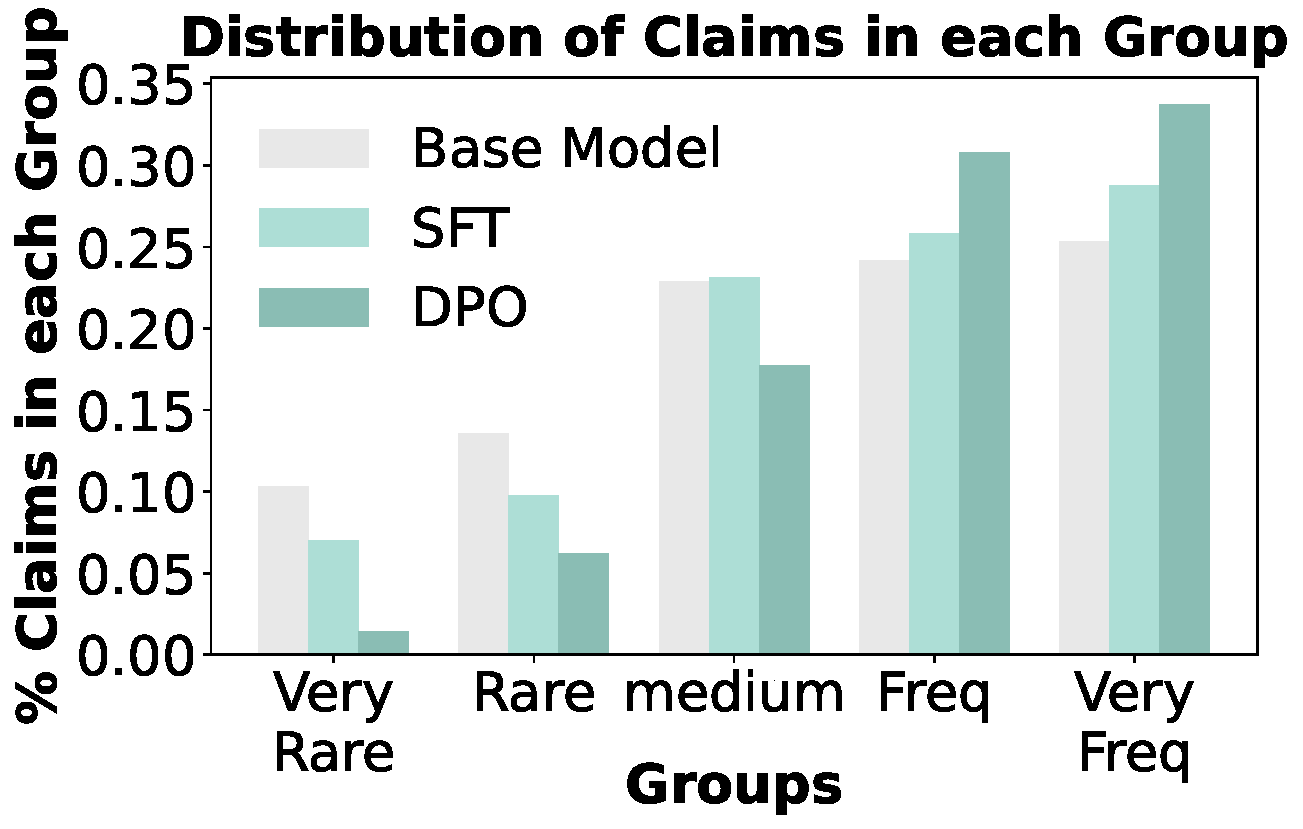
\includegraphics[width=\textwidth]{FenCE_figures/distribution_claims_by_group.pdf}
    \caption{Distribution of claims}
    \label{fig:response_shift_distribution_claims}
  \end{subfigure}
  \begin{subfigure}[b]{0.32\textwidth}
    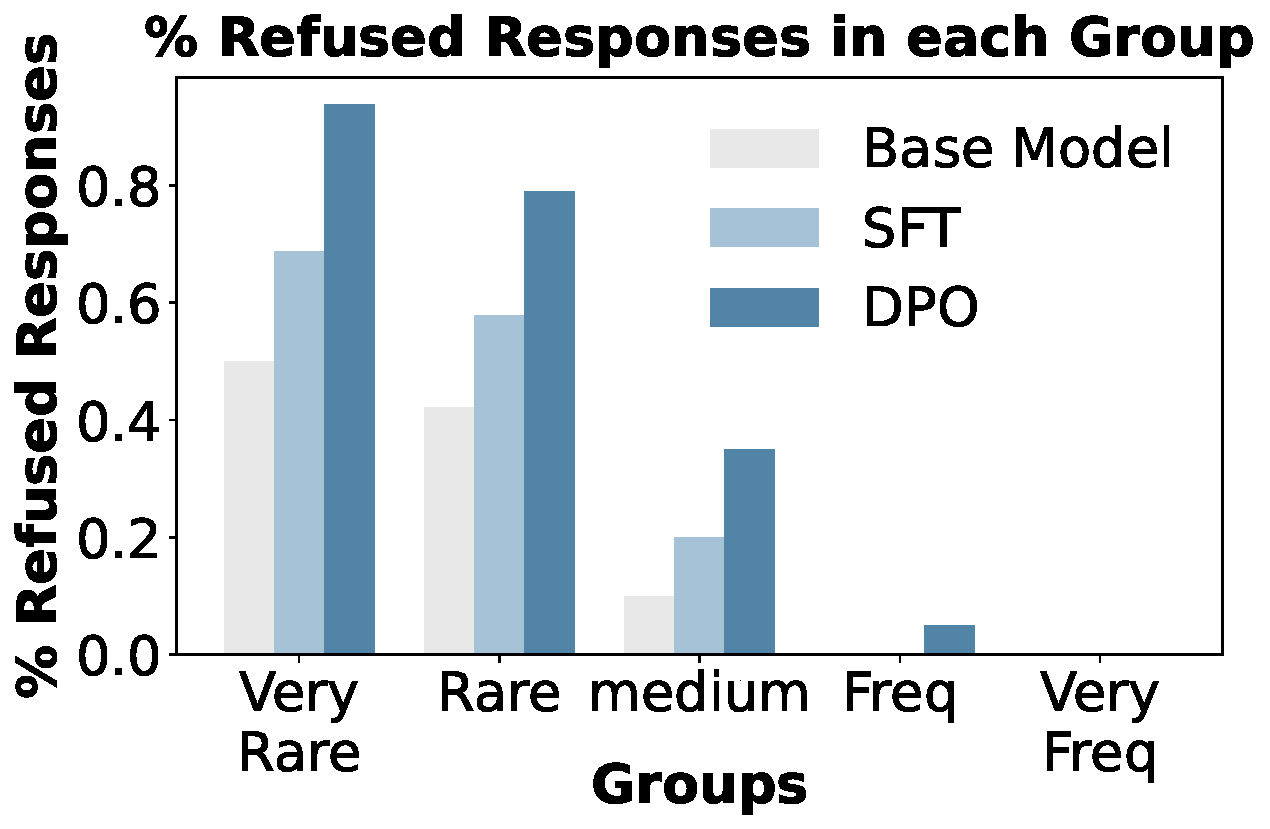
\includegraphics[width=\textwidth]{FenCE_figures/percent_refused_responses_by_group.pdf}
    \caption{\% Refused responses}
    \label{fig:response_shift_refused_responses}
  \end{subfigure}
  \begin{subfigure}[b]{0.32\textwidth}
    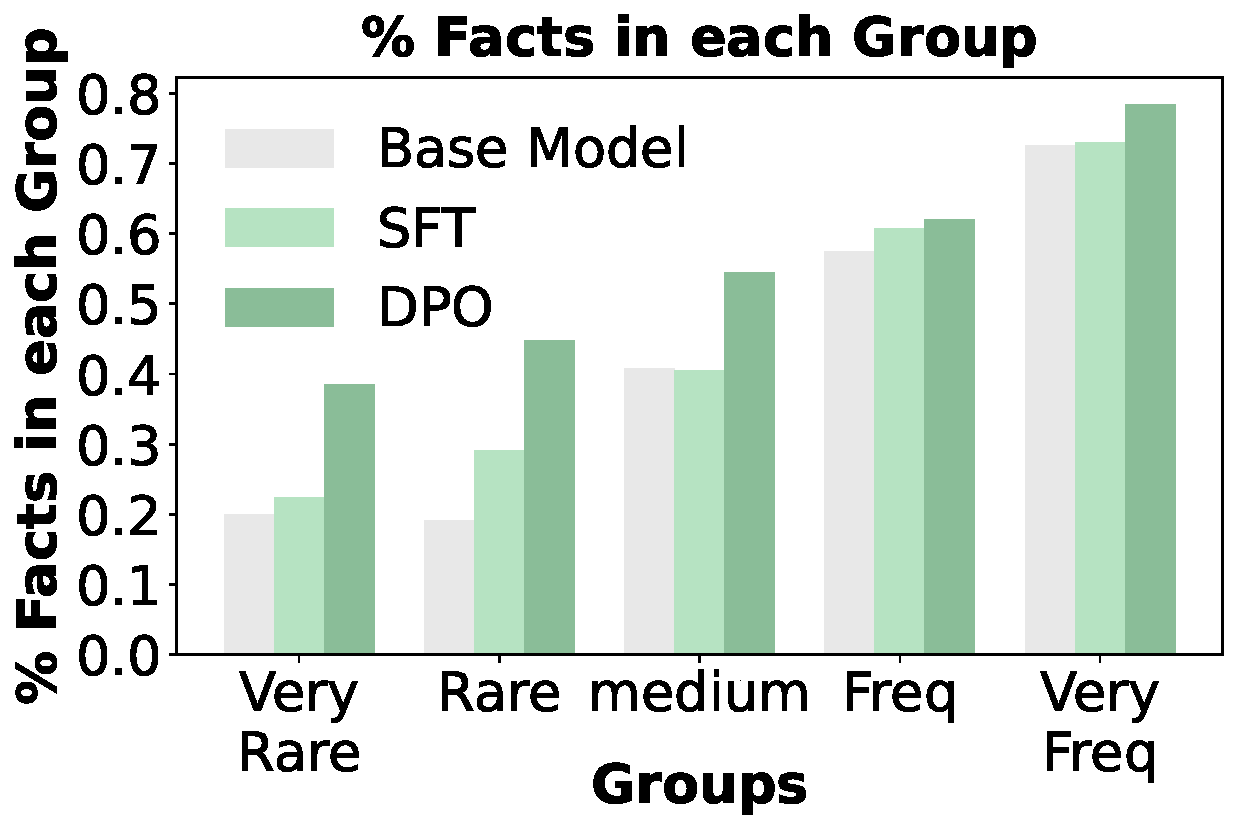
\includegraphics[width=\textwidth]{FenCE_figures/percent_facts_by_group.pdf}
    \caption{\% Facts}
    \label{fig:response_shift_num_facts}
  \end{subfigure}
  
  \caption{Statistics of generated responses, where we group the prompts by the popularity of the person to write biography for, as labeled in the FActScore dataset. We compare zero-shot Llama3-8B-chat (denoted as \textit{``Base Model''}), SFT + \fencemodelname (\textit{``SFT''}), and our method, Edit/Remove + Coarse (\textit{``DPO''}).}
  \label{fig:response_shift}
\end{figure*}

\begin{figure}[t]
    \centering
    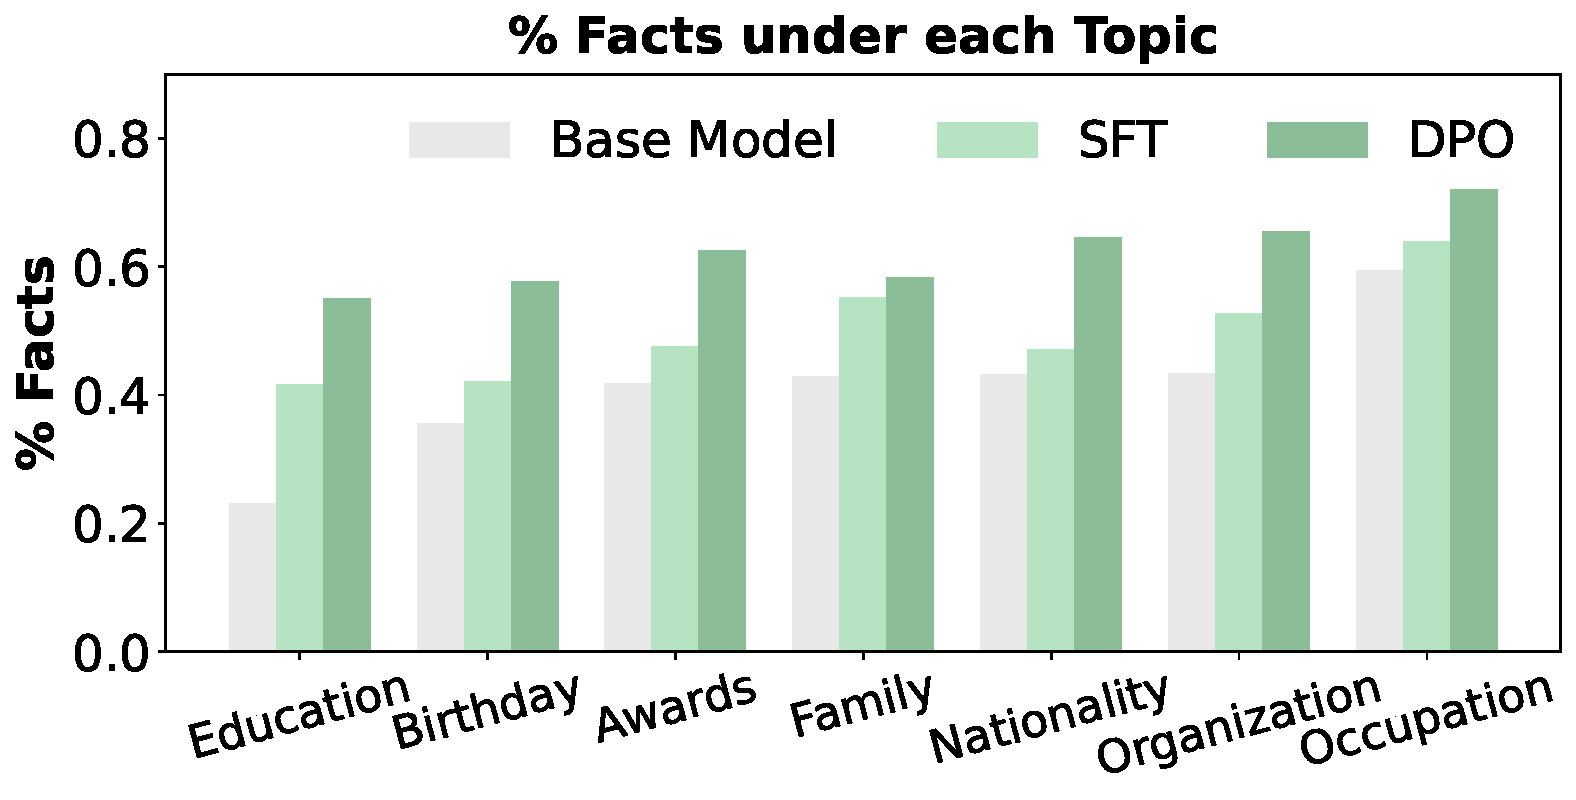
\includegraphics[width=0.7\linewidth]{FenCE_figures/facts_by_cat.pdf}
    \upv
    \caption{The factuality of claims with different topics, where we pre-define the topics and use Llama3-70B-chat to predict whether each claim covers any topic(s).}
    \label{fig:claim_acc_by_cat}
    \downv
\end{figure}



\start{Baselines and Ablations}
We implement four baselines: SFT, FactTune-FS~\citep{FactTune}, Self-Eval-SKT~\cite{self-eval-skt}, and EVER-Pref~\citep{EVER}. 
All methods sample $N$ candidate responses for each training prompt.
SFT first uses the generator itself to score responses by computing the percentage of factual claims and finetunes with the best response.
FactTune-FS first finetunes on all candidates and then uses all $\binom{N}{2}$ candidate pairs as DPO pairs, preferring the one with a higher score based on retrieved context.
Self-Eval-SKT self-trains an evaluator using the model's own knowledge and uses the evaluator to score responses with no external context, also resulting in $\binom{N}{2}$ preference pairs.
EVER-Pref uses all $N$ candidates as rejected responses and constructs a preferred response by iteratively evaluating and correcting false information in each passage.

For ablations, we first equip SFT, FactTune, and EVER with our evaluator, \fencemodelname, and the three external tools, denoted as ``SFT + \fencemodelname'', ``Coarse'', and ``Edit'' in \autoref{tab:res-ablation}, respectively. 
Then we implement ``Edit + Coarse'', which corrects all false information without checking whether it corresponds to a lesser-known fact.
We denote our full method as ``E/R + Coarse'' (Edit/Remove + Coarse).
% More implementation details can be found in \S\ref{sec:implementation_details}.

Note that we do not compare to retrieval-augmented (RAG) methods~\cite{RAG} because it is not a fair comparison. RAG-based methods require access to external knowledge sources or tools in inference, while in our experiments, we only used ``\texttt{tell me a bio of <entity>}'' as the prompt. 
Furthermore, while most RAG-based methods aim to improve the understanding of the long retrieved context, our main focus is to train the model to better utilize the knowledge it has seen during pretraining.

We also do not compare to inference-time methods~\cite{ITI,DoLA} because these methods need to call the model multiple times in inference, introducing heavy latency issues. In the real world, such latency is unacceptable in production. In comparison, our method uses the standard random decoding in inference and does not introduce extra inference-time cost. Furthermore, in principle, our method is orthogonal to those inference-time methods and can be combined.


\begin{figure}[t]
  \centering
  % \hspace{-0.4cm}
  \begin{subfigure}[b]{0.4\textwidth}
    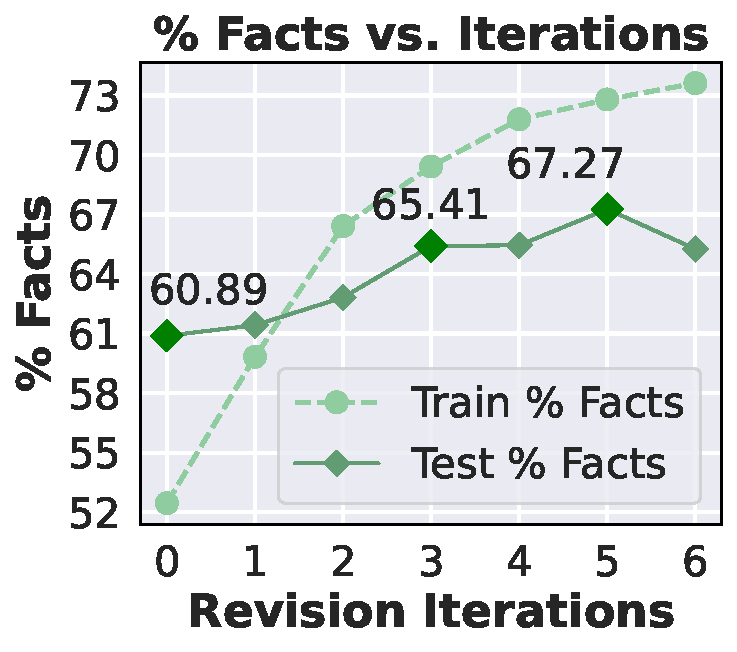
\includegraphics[width=\textwidth]{FenCE_figures/hyper_param.pdf}
    % \vspace{-0.5cm}
    \caption{Iterations of Revision}
    \label{fig:hyper_param_iter}
  \end{subfigure}
  \hspace{0.4cm}
  \begin{subfigure}[b]{0.375\textwidth}
    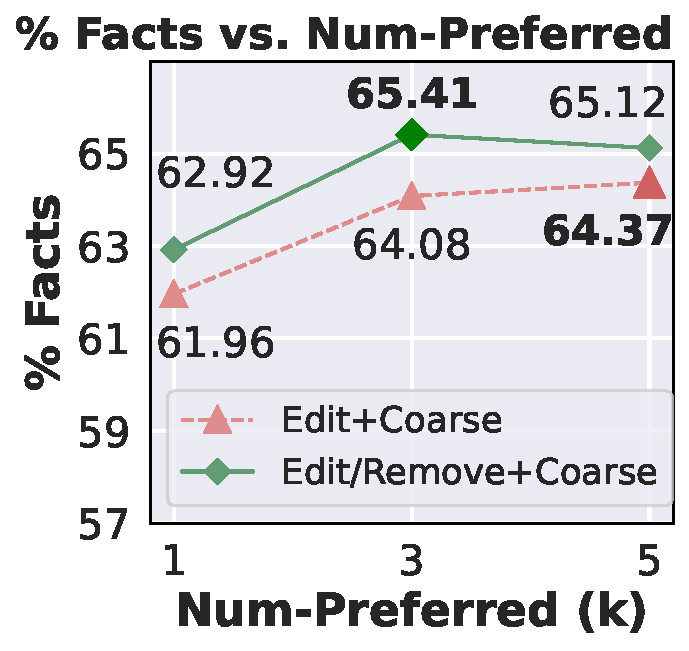
\includegraphics[width=\textwidth]{FenCE_figures/hyper_param_topk.pdf}
    % \vspace{-0.5cm}
    \caption{top-$k$}
    \label{fig:hyper_param_k}
  \end{subfigure}
  \caption{Hyper-parameter analysis. We investigate how percentage of facts changes
  (a) as number of iterations to revise candidate responses increases, and 
  (b) with different numbers of preferred responses for each prompt.
  }
  \label{fig:hyper-param}
\end{figure}

\subsection{Main Results}
Results in \autoref{tab:res-factscore} answer (\textbf{RQ2}) and show that our method significantly improves Llama2/Llama3's factuality by 16.85/14.45\% on FActScore and 17.64\%/8.25\% on TruthfulQA.
Results also show that our method significantly outperforms the best baseline on factuality training (e.g., by 8.83/6.96\% on FActScore for Llama2/Llama3).

\autoref{tab:res-ablation} presents the ablations with \fencemodelname as the evaluator.
The comparison between using \fencemodelname and Llama3-8B-chat shows that \fencemodelname can improve the performance of SFT, EVER-Pref, and FactTune-FS, which emphasizes the significance of training factuality evaluator models.
For example, SFT with \fencemodelname as the evaluator outperforms SFT with Llama3 as the evaluator by 3.74\%.
In addition, we also observe that our method of combining response editing/removing with coarse-level scoring achieves significantly better performance.
% In particular, our full method, which only corrects false information with common facts, outperforms ``Edit + Coarse'', which could introduce both common and lesser-known facts into the training data.
The above results answer (\textbf{RQ3}), demonstrating the effectiveness of our training recipe.






\subsection{Result Analyses}

\start{Distribution of Generated Claims}
We first group the prompts by the popularity of the person to write biography for, which is provided as meta data in the FActScore dataset, and then compare the distribution of generated claims in each group before and after training.
As shown in \autoref{fig:response_shift_distribution_claims}, after training, the generator outputs less information for unfamiliar people and outputs more information for popular ones, suggesting that it learns to only generate information that is likely to be factual.

In addition, as shown in \autoref{fig:response_shift_refused_responses}, we observe that the generator refuses to generate responses more frequently for rare entities (e.g., by generating ``I apologize, but I'm not familiar with this person.''), and almost never refuses for frequent ones. 
This aligns with previous research's conclusion~\citep{unfamiliar-finetuning} that training the model to say ``I don't know'' to unfamiliar prompts reduces hallucination.


\start{Performance Breakdown}
We further check the generator's performance (i.e., percentage of factual claims) on different groups of prompts. 
As shown in \autoref{fig:response_shift_num_facts}, we observe that our method achieves consistent performance gain over all groups of prompts, which is another reason why our method obtains higher overall performance.

Similarly, we check the performance on claims describing different topics, where we first come up with a list of topics and then prompts Llama3-70B-chat to determine whether each claim covers any of the topics. 
In \autoref{fig:claim_acc_by_cat}, our method generates more factual claims under all the topics, and the performance gain is larger on unfamiliar topics (i.e., topics where the generator has lower scores). 

\start{Hyper-parameter Analysis}
We first alternate the number of iterations to revise the responses and inspect the testing and training accuracy (i.e., the average \% of facts of the best preferred responses).
As shown in \autoref{fig:hyper_param_iter}, with more revision iterations, we can always obtain preferred responses with better factuality, but the test performance converges after the third iteration. 
In other words, training data with fewer factual errors does not always transfer to better test performance.


In our experiments, we only choose the top-$k$ candidates (ranked by the percentage of facts) as preferred responses. We investigate the effect of $k$ in \autoref{fig:hyper_param_k}. We observe that training on top-3 and top-5 responses leads to similar performance. With all the $k$s in our experiments, our method consistently outperforms the ``Edit + Coarse'' ablation.




% \section{Related Work}
% \start{Factuality Evaluation} To judge the factuality of long-form model responses, recent works have presented fine-grained level evaluation frameworks that judge each piece of generated fact individually~\citep{factscore,factool,doclens,longform}.
% Such frameworks generally leverage an LM evaluator to make judgments.

% To train LM evaluators, one line of work constructs new training datasets by collecting human judgement~\citep{alpaca_eval,TIGERScore}. 
% Another line of work distills open-source evaluators from proprietary models such as GPT-4, training the evaluator to generate textual critique~\citep{shepherd,ultrafeedback,AutoJ} or fine-grained judgment~\citep{prometheus,FAVA}.
% A recent work \citep{FLAMe} leverages a combination of existing public datasets to train an evaluator.
% We further augment the public datasets with more diverse knowledge sources and more informative judgment feedback.


% \start{Enhancing Generator's Factuality}
% To reduce hallucinations, previous works present inference-time methods, including re-computing token probabilities~\cite{CAD,DoLA} or conducting post-editing~\cite{self-critiquing,self-improve,self-correct,self-refine,CRITIC,FAVA}. Such methods inevitably suffer from latency issues.

% Another approach is to train the model for factuality. Following general reward modeling methods that produce a score for the entire response~\citep{RLHF,InstructGPT,RLHF-QA}, FactTune \citep{FactTune} trains the generator by preferring responses with higher percentage of facts, which is limited by the generator's capability. 
% EVER~\citep{EVER} constructs high-quality responses by correcting false information, which may introduce lesser-known facts and could potentially harm model factuality~\citep{understand-finetuning}.
% Both methods either prompt proprietary model or use the generator itself to evaluate its own factuality, which are either restricted by terms of use or suffer from self-bias.

% Our method is different from existing methods in the following aspects: (1) we combine response revision and scoring to construct high-quality responses while ensuring the correctness of preference ranking, (2) we only correct false information with common facts and remove other misinformation from training, and (3) we use our open-source evaluator, \fencemodelname, for both revision and scoring.




\section{Chapter Summary}
In this chapter, we improve LM generators' factuality by training an open-source evaluator model, \fencemodelname.
To train \fencemodelname to leverage diverse knowledge sources and to generate more informative feedback, 
we equip a combination of public datasets with textual critique along with judgment scores and obtain additional source documents by calling a multiplicity of tools.
We then present a training recipe that leverages \fencemodelname to finetune LM generators for better factuality, where we construct preference data by prompting \fencemodelname to revise and score the generator's responses, without introducing lesser-known facts in training.
Experiments show that \fencemodelname outperforms strong proprietary models such as Claude-3 on LLM-AggreFact.
Our factuality training method improves Llama3-8B-chat's factuality performance by 14.45\% on FActScore and 8.25\% on TruthfulQA.

\autoref{chap:prm-training} adapts the high-level idea of auxiliary model training to coding agent, where we first show that the coding agent performs better in inference if it receives critique from an auxiliary model every $k$ steps. Then, we propose a data construction method to train an open-source critique model. 



\begin{table*}[!t]
\centering

\resizebox{\textwidth}{!}{
\begin{tabular}{p{20.1cm}}
\toprule
\dlrow \textit{\textbf{Source Document} (Dataset: FRANK-xsum)}  \\
Title: News Articles \\
Text: They believe ministers are placing too much emphasis on the environment at the expense of trees grown for timber.
Britain is currently the world's third largest importer of wood.
Ministers said they were encouraging commercial forestry organisations to invest in woodland creation.
Conifer forests have been a familiar sight for half a century in Wales and have helped the timber industry grow.
But Confor, which promotes the forestry industry, warns that at least 16,000 hectares - or 40,000 acres - of commercial forest have been lost since 2001 and need to be re-planted to meet needs.
Half of the woodland is managed by Natural Resources Wales with the the other half by private companies.
As an industry, it is estimated to be worth more than £450m a year to the Welsh economy.
But there is a conflict with environmental policy.
\textbf{Successive ministers have wanted more native, broadleaf species of trees and better access for walkers and bike riders while conservationists claim commercial forests are bad for wildlife.}
However, some forests in Wales are difficult to reach and hard to harvest while transporting the timber through rural communities can bring companies into conflict with local residents.
The Welsh government wants a balance between the environmental, the economic and the social in how forestry is developed.
It points to its Glastir scheme which encourages farmers and other landowners to plant woodland.
It said its Woodlands for Wales forestry strategy "sets out how we want Wales to be known for its high quality woodlands that enhance the landscape, provide real social and community benefits, support thriving woodland-based industries and contribute to a better quality environment".
Martin Bishop, of Confor, which represents 200 businesses in Wales, believes the emphasis on environmental aspects is seen as "sexier" than commercial forestry.
He said the current system is also too bureaucratic for creating new woodland areas.
Mr Bishop said 90 hectares were planted last year but there needed to be 20,000 hectares a year to meet long-term targets set by ministers.
"There's a huge market for our timber. Every saw miller tells me he would double or treble production if the timber was there to feed that mill," he added. \\
\\
\midrule 

\dlrow \textit{\textbf{Claim}} \\
Conservationists are calling for a national project to protect forests in wales. \\
\\
\dlrow \textit{\textbf{Ground Truth Label}} \\
\colorR{Non-Factual} \\
\\
\midrule

\blrow \textit{\textbf{Our Generated Critique and Label}} \\
\textbf{Critique}: The document does not mention conservationists calling for a national project to protect forests in Wales. It only mentions that conservationists claim commercial forests are bad for wildlife, but it does not mention a specific call for a national project. \\
\\
\textbf{Label}: \colorR{Unverified} \\
\bottomrule
\end{tabular}
}
% \vspace{-0.05cm}
\caption{An example of the textual critique we generate. We highlight the most relevant sentence in the document. In this case, our generated critique aligns with the judgment label.
}
\label{tab:case_1}
% \vspace{-0.2cm}
\end{table*}




\begin{table*}[!t]
\centering

\resizebox{\textwidth}{!}{
\begin{tabular}{p{24cm}}
\toprule
\dlrow \textit{\textbf{Original Source Document} (Dataset: FRANK-CNN/DM)}  \\ 
Title: News Articles \\
Text: (CNN) Deputies rushed Kenneth Morgan Stancil III from court Thursday after the 20-year-old murder suspect swore at a judge and tried to flip over a table. Stancil is accused of killing an employee Monday at Wayne Community College in Goldsboro, North Carolina. Relatives have said victim Ron Lane was gay, CNN affiliate WNCN reported, and investigators are looking into whether the shooting was a hate crime. Authorities arrested Stancil after he was found sleeping on a Florida beach on Tuesday. Just a few minutes into Thursday's hearing on the first-degree murder charge he faces, Stancil snapped back at the judge after he was offered a court-appointed lawyer. \"No, I don't need one,\" said Stancil, who stood before the judge with his legs shackled and his arms handcuffed in front of him. \"You know what I'm saying? I knew I would get life anyway.\" Superior Court Judge Arnold O. Jones interjected, pointing out that the maximum sentence Stancil faces is the death penalty. \"Yes, I know that,\" Stancil fired back. \"But when I knew what I had to do and I knew when I got caught, you know, I knew in my mind that I could get life, I could get the death penalty. You know what I'm saying? Do you follow my topic? I would have killed you, you know what I'm saying, if you're a f---ing child molester.\" The judge told him not to swear. \"I don't give a f--- what you want,\" Stancil said, lunging forward and lifting up the table in front of him. Deputies quickly corralled him and hustled him from the courtroom. The hearing resumed about 25 minutes later, when Stancil was brought back into the courtroom, this time with his arms handcuffed behind him. When asked again by Jones whether he wanted a lawyer, his response was quick -- and calm. \"Yes, sir,\" he said. In an interview with CNN affiliate WRAL, Stancil described himself as a neo-Nazi and said he hates gay people \"with a passion.\" Stancil had worked for Lane, the school's print shop operator, as part of a work-study program, but was let go from the program in early March because of poor attendance, college officials said. \\
\\
\midrule 

\dlrow \textit{\textbf{Claim}} \\
Kenneth Morgan Stancil is accused of killing an employee at Wayne Community College in Goldsboro, North Carolina. \\
\\
\dlrow \textit{\textbf{Ground Truth Label}} \\
\colorG{Factual} \\
\\
\midrule

\blrow \textit{\textbf{Generated Queries to Call the Tools}} \\
\textbf{Search query for Bing Search API}: Kenneth Morgan Stancil Wayne Community College killing \\
\textbf{Queries for Wikipedia}: Kenneth Morgan Stancil; List of school shootings in the United States; Wayne Community College; \\
\textbf{Entities for Google Knowledge Graph API}: Kenneth Morgan Stancil \\
\\
\midrule

\blrow \textit{\textbf{Tool-extracted Source Documents} (after Reranking)} \\
Title: Wayne Community College shooter gets life sentence without parole \\
Text: GOLDSBORO, North Carolina (WTVD) -- \textbf{Kenneth Morgan Stancil III was sentenced Tuesday to life in prison without parole for the murder of 44-year-old Ron Lane on the campus of Wayne Community College in Goldsboro on April 13, 2015.}
Stancil entered the campus print shop on the third floor of the same building that houses the school library and cafeteria shortly after Lane arrived for work that day and shot him once with a pistol-grip 12-gauge shotgun.
...
\\
\\
Title: Stancil guilty in Wayne Community College murder trial - CBS17.com \\
Text: GOLDSBORO, N.C. (WNCN) – After deliberating for an hour and a half, \textbf{a Wayne County jury found Kenneth Morgan Stancil III guilty of first-degree murder.}
He will spend the rest of his life in prison.
During his closing argument Tuesday in a Wayne County court, the district attorney relied largely on Stancil’s own words, \textbf{painting him as confident and proud about his decision to kill a man at Wayne Community College.}
In his counterargument, Stancil’s attorney said the prosecution tried to scare the jury with Stancil’s possession of knives, guns, and white supremacist memorabilia, as well as his numerous tattoos. None of that proved he planned to commit the murder, the defense said.
\textbf{Neither side disputed that Stancil killed Ron Lane at Wayne Community College in 2015}. The prosecution contends it was first-degree murder, but the defense argues ...
\\
\\
Title: Man convicted in fatal Wayne Community College shooting - WRAL ... \\
Text: Man convicted in fatal Wayne Community College shooting
A white supremacist was sentenced Tuesday to life in prison without parole for gunning down a print shop operator at Wayne Community College two years ago.
\textbf{Jurors deliberated for about 90 minutes before convicting Kenneth Morgan Stancil III, 22, of first-degree murder in the April 13, 2015, death of Ron Lane in the school's library.}
Authorities said Stancil shot Lane with a 12-gauge pump shotgun before fleeing the area on a motorcycle. He was captured the next morning when police found him asleep on a beach in Volusia County, Fla.
...
\\
\\
Title: Wayne Community College killing suspect makes shocking allegations in ... \\
... \\
\midrule

\blrow \textit{\textbf{Our Generated Critique and Label}} \\
\textbf{Critique}: The statement is supported by the document. In all the documents, it is mentioned that Kenneth Morgan Stancil III is accused of killing Ron Lane, an employee at Wayne Community College in Goldsboro, North Carolina. \\
\\
\textbf{Label}: \colorG{Supported} \\
\bottomrule
\end{tabular}
}
% \vspace{-0.05cm}
\caption{An example where we obtain multiple relevant source documents by calling a multiplicity of tools.
}
\label{tab:case_2}
% \vspace{-0.2cm}
\end{table*}




\begin{table*}[!t]
\centering

\resizebox{\textwidth}{!}{
\begin{tabular}{p{21cm}}
\toprule
\dlrow \textit{\textbf{Original Source Document} (Dataset: FActScore)}  \\ 
Title: Chadwick Boseman \\
Text: Chadwick Boseman Chadwick Aaron Boseman \textbf{(; November 29, 1976August 28, 2020)} was an American actor. During his two-decade career, Boseman received multiple accolades, including two Screen Actors Guild Awards, a Golden Globe Award, a Critics' Choice Movie Award, a Primetime Emmy Award, and an Academy Award nomination. After studying directing at Howard University, Boseman began his career in theatre, winning a Drama League Directing Fellowship and an acting AUDELCO ...
\\
\\
\midrule 

\dlrow \textit{\textbf{Claim}} \\
Chadwick Boseman was born on November 29, 1977. \\
\\
\dlrow \textit{\textbf{Ground Truth Label}} \\
\colorR{Non-Factual} \\
\\
\midrule

\blrow \textit{\textbf{Generated Queries to Call the Tools}} \\
\textbf{Search query for Bing Search API}: Chadwick Boseman date of birth \\
\textbf{Queries for Wikipedia}: Chadwick Boseman \\
\textbf{Entities for Google Knowledge Graph API}: Chadwick Boseman Stancil \\
\\
\midrule

\blrow \textit{\textbf{Tool-extracted Source Documents} (after Reranking)} \\
Title: knowledge graph result \\
Text: Chadwick Boseman: American actor. Chadwick Aaron Boseman was an American actor, known for portraying African-American historical figures and the fictional African superhero Black Panther. \textbf{Chadwick Boseman Born: November 29, 1976, Anderson, SC.} Chadwick Boseman Died: August 28, 2020 (age 43\u00a0years), Los Angeles, CA. Chadwick Boseman Spouse: Taylor Simone Ledward. Chadwick Boseman Height: 6\u2032 0\u2033. Chadwick Boseman Parents: Leroy Boseman and Carolyn Boseman. Chadwick Boseman Alma mater: Howard University (BFA).
...
\\
\\
Title: Chadwick Boseman | Biography, Movies, Black Panther, \& Death
text: Chadwick Boseman \\
Text: Our editors will review what you’ve submitted and determine whether to revise the article. \\
- Chadwick Aaron Boseman \\
\textbf{- Born: November 29, 1976, Anderson, South Carolina, U.S.} \\
- Died: August 28, 2020, Los Angeles, California (aged 43) \\
- Notable Family Members: son of Leroy Boseman ... \\
Chadwick Boseman (born November 29, 1976, Anderson, South Carolina, U.S.—died August 28, 2020, Los Angeles, California) was an American actor and playwright who became a highly respected movie star with several iconic roles, notably that of T’Challa/Black Panther in the groundbreaking film Black Panther (2018).
...
\\
\\
Title: Chadwick Boseman - Wikipedia \\
Text: Chadwick Boseman Chadwick Aaron Boseman \textbf{(; November 29, 1976August 28, 2020)} was an American actor. During his two-decade career, Boseman received multiple accolades, including two Screen Actors Guild Awards, a Golden Globe Award, a Critics' Choice Movie Award, a Primetime Emmy Award, and an Academy Award nomination. After studying directing at Howard University, Boseman began his career in theatre, winning a Drama League Directing Fellowship and an acting AUDELCO ...
\\
\\
Title: Chadwick Boseman | Biography, Movies, Black Panther, \& Death ... \\
... \\
\midrule

\blrow \textit{\textbf{Our Generated Critique and Label}} \\
\textbf{Critique}: The statement claims that Chadwick Boseman was born on November 29, 1977. However, all four documents consistently state that Chadwick Boseman was born on November 29, 1976, not 1977. \\
\\
\textbf{Label}: \colorR{Contradictory} \\
\bottomrule
\end{tabular}
}
% \vspace{-0.05cm}
\caption{An example where we obtain multiple relevant source documents by calling a multiplicity of tools. The tool-extracted documents all contain the information about Chadwick's birthday, but have diverse formats.
}
\label{tab:case_3}
% \vspace{-0.2cm}
\end{table*}









\chapter{Improving Coding Agent Effectiveness by Training a Critique Model \textcolor{mediumgreen}{(\textit{proposed})}}
\label{chap:prm-training}

\section{Overview}
Synthetic data has proven effective for training coding agents~\cite{swe-smith,R2EGym,hybrid-gym}. However, as in many machine learning settings, the effectiveness of a coding agent is ultimately bottlenecked by the capacity of its base model. Prior work~\cite{swe-smith} shows that, when using Qwen2.5Coder-14B as the base model, coding-agent performance already saturates after roughly 800 training trajectories.

To overcome this limitation, we propose training an auxiliary model to assist the coding agent at inference time. Similar to \autoref{chap:fence}, an ideal auxiliary model should satisfy two properties: (1) it should provide additional performance gains when paired with the primary coding agent, and (2) it should develop capabilities that differ from those of the main coding agent, allowing the two models to be optimized for distinct objectives.

In this chapter, we show that a critique model trained to provide free-form textual feedback to the main model during inference satisfies both criteria for coding-agent tasks. Using a strong critique model such as Claude-Sonnet-4.6, we improve the performance of CWM-32B~\cite{cwm} on SWE-Bench Verified-mini~\cite{swebench} from 29.4\% to 61.0\%. Moreover, we find that using a model fine-tuned for coding-agent tasks, such as SWE-Smith-7B~\cite{swe-smith}, as the critique model does not yield additional gains beyond those achieved by the coding agent alone. This suggests that the critique model requires a different set of capabilities and should be optimized differently from the coding agent itself.

Because using a frontier model as the critique model, such as Claude-Sonnet-4.6, remains expensive at inference time, our \textcolor{aquablue}{\textbf{preliminary experiments}} focus on constructing synthetic data to distill a more cost-efficient critique model, such as Qwen3-8B, that can provide free-form textual critiques to assist the main coding agent during inference. Specifically, we distill Qwen3-8B from Claude-generated critiques using standard supervised fine-tuning (SFT), and this already improves CWM-32B's performance on SWE-Bench Verified from 29.4\% to 33.4\%.

However, we observe that the fine-tuned critique model does not fully reproduce the behavior of the frontier critique model. In particular, its critiques tend to be more verbose, repeating, and contain more unnecessary details, which can distract the main coding agent. These distractions often lead the agent to take unnecessary actions and exhaust the budget of action steps before producing a valid code patch.
In particular, we observe that the vanilla coding agent generates an non-empty code patch for 89.0\% of the examples in SWE-Bench Verified, but when paired with the SFT critique model, the non-empty rate is significantly reduced to 73.4\%.
This indicates that reducing distracting critiques and improving the non-empty rate could be a promising direction to further improve the performance of the system.

Motivated by these observations, we \textcolor{mediumgreen}{\textbf{propose}} to (1) systematically analyze the characteristics of distracting critiques that lead to unnecessary actions, and (2) construct direct preference optimization (DPO) data to further improve the critique model by encouraging it to generate fewer distracting critiques.


\section{Preliminary Experiments}
In our preliminary experiments, we first show that a strong critique model can bring substantial performance gains to the coding agent in inference (\S\ref{sec:prm-strong}).
Then we show that we can further train a more cost-efficient critique model (e.g., Qwen3-8B) by distilling it from the strong critique model (e.g., Claude-Sonnet-4.6) using vanilla supervised-finetuning (SFT) (\S\ref{sec:prm-sft}).
Finally, we reveal the remaining gaps between the student critique model and the teacher critique model, which motivates our proposed method (\S\ref{sec:prm-proposed}).

\subsection{Inference-time Critique Models can be Effective}
\label{sec:prm-strong}

\start{Experimental Setup}
We experiment with the SWE-Bench Verified dataset~\cite{swebench} with mini-SWE-Agent as the infrastructure~\cite{sweagent}. We use CWM-32B~\cite{cwm} as the coding agent and experiment with three critique models: a frontier model, Claude-Sonnet-4.6~\cite{claude46}, a cost-efficient open-source model, Qwen3-8B~\cite{qwen3}, and a model finetuned for coding agent tasks, SWE-Smith-7B~\cite{swe-smith}.

Following previous work~\cite{swe-prm}, we adopt the setting where the critique model provides free-form textual critique for the main coding agent every $k$ steps during inference. We use $k=5$ in our experiments. The coding agent can perform at most $150$ steps. After exceeding the limit, the process will be terminated, even if no coding patch is generated.

We prompt the critique model to include (1) error analysis for the current trajectory, (2) high-level instructions for completing the task, and (3) the reasoning process for generating the critique, which is shown to be effective empirically~\cite{swe-prm}. 

\start{Experimental Results}
As shown in \autoref{tab:prm:prelim}, we observe that:
(1) The frontier critique model (Claude-Sonnet-4.6) can bring substantial performance gains to the coding agent, improving the resolved rate from 29.4\% to 61.0\%.
(2) Using a weak critique model such as Qwen3-8B may even reduce the performance of the coding agent, but the performance loss is not significant.
(3) The model finetuned for coding agent tasks (SWE-Smith-7B) is not an effective critique model, which performs even worse than Qwen3-8B. This indicates that the critique model and the coding agent require different capabilities and should be optimized differently.



\begin{table}[t]
  \centering
  \small
  \resizebox{0.6\columnwidth}{!}{%
  \begin{tabular}{l ccc}
  \toprule
  \multirow{2}{*}{\bf Crtique Model} &
  \multicolumn{3}{c}{\bf SWE-Bench Verified} \\
  \cmidrule(lr){2-4}
  & Resolved \% & Non-Empty \% & Avg Steps \\
  \midrule
  \sdlrow & \multicolumn{3}{c}{\textit{Coding Agent: CWM-32B}} \\
  \midrule
  \textemdash & 29.4 & 89.0 & 34.54 \\
  \midrule
  Qwen3-8B & \bad 24.6 & 82.4 & 39.57 \\
  SWE-Smith-7B & \bad 21.2 & 62.2 & 41.07 \\
  Claude-Sonnet-4.6   & \better \bf 61.0 &  90.0 & 30.28 \\
  \midrule
  Qwen3-8B + SFT & \good 33.4 & 73.4 & 61.39 \\
  \quad + fallback & \good 36.4 & 94.8 & \textemdash \\
  \bottomrule
  \end{tabular}%
  }
  \caption{Results on equipping CWM-32B with different critique models on SWE-Bench Verified. ``fallback'' refers to the setting where if the coding agent exceeds the limit, we run inference on this example again without the critique model.}
  \label{tab:prm:prelim}
\end{table}


\subsection{Distilled Critique Models also Bring Performance Gains}
\label{sec:prm-sft}
\start{Experimental Setup}
To reduce inference cost, we distill Qwen3-8B from Claude-Sonnet-4.6 using vanilla supervised-finetuning (SFT).

We build training data from 500 trajectories with CWM-32B as the coding agent and Claude-Sonnet-4.6 as the critique model. For each piece of critique, we use the partial trajectory before it as the prefix and optimize the probability of the critique.

We train the model on 8 L-40 GPUs, with a batch size of 8, and a learning rate of 5e-6. We train the model for 3 epochs.

\start{Experimental Results}
As shown in \autoref{tab:prm:prelim}, we observe that the SFT model can also bring performance gains to the coding agent, improving the resolved rate from 29.4\% to 33.4\%.
However, the performance gap with using the frontier critique model is still large, indicating that there is still a large room for improvement.

\start{The Remaining Gaps}
We observe that one major reason that limits the performance of the SFT-critique model is that is has a much lower non-empty rate than the base coding agent (reducing from 89.0\% to 73.4\%). What happens is that when the critique is distracting, the coding agent performs on average more actions than before (increasing from 34.54 to 61.39). It exceeds the limit of 150 steps more often, where the process is terminated before a valid code patch is generated.

We present a simple fix to the limit-exceeding problem denoted as ``+ fallback'' in \autoref{tab:prm:prelim}. Specifically, when the coding agent exceeds the limit, we start from the first step again and run inference with the coding agent alone, without any critique models. This improves the non-empty rate from 73.4\% to 94.8\% and improves the resolved rate from 33.4\% to 36.4\%.

However, to reduce inference latency, we aim to train the critique model itself to avoid distracting behaviors. In the next section, we propose to systematically investigate the characteristics of the distracting critiques that lead to unnecessary actions, and construct training data to reduce such distracting behaviors.



\section{Proposed Method}
\label{sec:prm-proposed}

\subsection{Analysis of Distracting Critiques}
\start{Proposed Method}
To investigate what types of critiques are distracting and lead to unnecessary actions, we propose to manually check a subset of trajectories where using the SFT critique model exceeds the limit but using Claude-4.6 as the critique model does not, and discover a list of differences between the critiques they generate.

Below is a list of differences that we already observed. Note that the list is not complete and will be updated as we conduct further analysis.
\begin{itemize}
  \item \textbf{The SFT critique model generates more implementation-level suggestions and the frontier model generates more high-level instructions}. For instance, the SFT critique model generates the concrete commands to execute, while the frontier model generates the general plan to locate the relevant files or fix the issue. We observe that when provided with implementation-level guidance, the coding agent tends to follow the exactly same suggestions in the critique. When the critique is distracting, the coding agent performs more unnecessary actions than before and exceeds the limit more often. Furthermore, the training data for the critique model contains much fewer concrete actions than the coding agent model. In this way, it is likely that the critique model has weaker action generation capability than the coding agent, making it unreasonable for the coding agent to follow its suggested actions.
  \item \textbf{The SFT critique model generates more complex critiques that contain more suggestions than the frontier model}. We observe that the SFT critique model tends to generate long critiques, while the frontier model generates shorter critiques and dynamically adjusts its suggestions based on the coding agent's progress.
  \item \textbf{The critique generated by the SFT model does not align well with the coding agent's recent progress}. We observe that there are cases where the SFT critique model generates the same instruction multiple times, even if the coding agent has already completed the first few steps in the instruction. In this way, the coding agent is likely to start over from the first step, stucking in a loop until the step limit is reached.
\end{itemize}

\start{Proposed Experiments}
In the next step, we propose to design controlled experiments to verify our hypothesis that the behaviors mentioned above are indeed harmful to the performance of the coding agent.

Specifically, for each type of behaviors that are potentially distracting, we use a frontier model to detect such critiques during inference. Whenever it observes such behaviors, we prompt the frontier model to revise the critique by removing such behaviors and keeping the remaining parts the same.
Then we compare the performance with the original and revised critiques.
If the revised critiques can bring significant performance gains, we can verify our hypothesis that such behavirors are indeed distracting and should be reduced from the critique.


\subsection{Constructing DPO Data to Distill Critique Models}
\start{Proposed Method}
After identifying the characteristics of the distracting critiques, we can construct directed preference optimization (DPO) data to further improve the performance of the critique model.

Similarly to the proposed analysis, we select ``breakpoints'' in the training trajectory, leverage the SFT critique model to generate multiple critiques, and prompt the frontier model to score the critiques based on whether they avoid the distracting behaviors. We will use the critiques with higher scores as the preferred responses and the critiques with lower scores as the rejected responses, and train the critique model with DPO.



\start{Proposed Experiments}
We expect to find that the DPO-trained critique model can generate fewer distracting critiques and improve the performance of the coding agent.

In particular, we evaluate the performance of coding agents on the SWE-Bench Verified dataset~\cite{swebench} with mini-SWE-Agent as the infrastructure~\cite{sweagent}.
We experiment on two base coding agents: CWM-32B~\cite{cwm} and Qwen2.5Coder-32B~\cite{qwen25coder}.
We expect to see that the performance of using the DPO-trained critique model is significantly better than three baselines and ablations: (1) inference with the coding agent alone, without any critique models,  (2) inference with the untrained model (Qwen3-8B or Qwen2.5Coder-32B) as the critique model, and (3) inference with the SFT-trained critique model.

